\section{System's Perspective}

\todo{Refferences?}

\subsection{Weekly Tasks Progress}
The weekly tasks, were based on the exercises that were given in the lecture. Tasks included implementing the features that were given in the lecture and having them ready before the next lecture, such that a release could be created.
\\\\
\textbf{Docker swarm}
The only weekly task that we did not implement was the Docker Swarm. We wanted to implement docker swarm into our Infrastructure as code script, but due to time constraints, we never had the opportunity to do so. 

\subsection{Design \& Architecture}
Frontend is built using Next.js\cite{nextjs}. The data is fetched through a Go Gin\cite{gin-gonic} API interacting with the database through an ORM called GORM\cite{gorm}. The service is deployed through Docker with the backend and frontend being separate containers. To provide insights into the system we also deploy "supporting" containers like EFK stack, Grafana \& Prometheus. Finally, we also have a container for Nginx responsible for providing a network configuration that allows us to have an SSL certificate along with a domain address.
\\\\
We chose Digital Ocean as our hosting provider using their VM service "Droplets". Our presence on digital ocean can be seen on \autoref{fig:do_infrastructure}. The system runs on a single droplet. We also pay for a hosted postgres database on Digital Ocean that we use to store all messages, follower relations and users. 

\begin{figure}[h!]
    \centering
    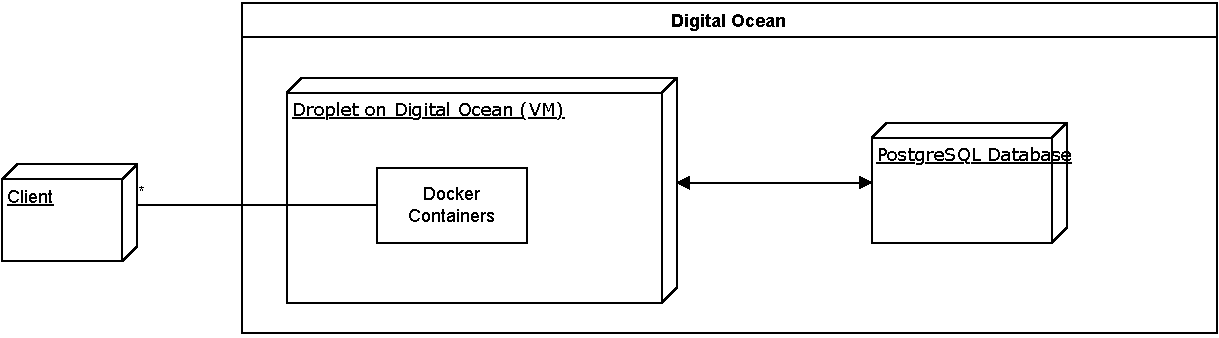
\includegraphics[scale=0.65]{diagrams/infrastructure.pdf}
    \caption{Digital Ocean infrastructure}
    \label{fig:do_infrastructure}
\end{figure}

An overview of the docker containers and their interactions are illustrated on \autoref{fig:docker_containers}.

\begin{figure}[H]
    \centering
    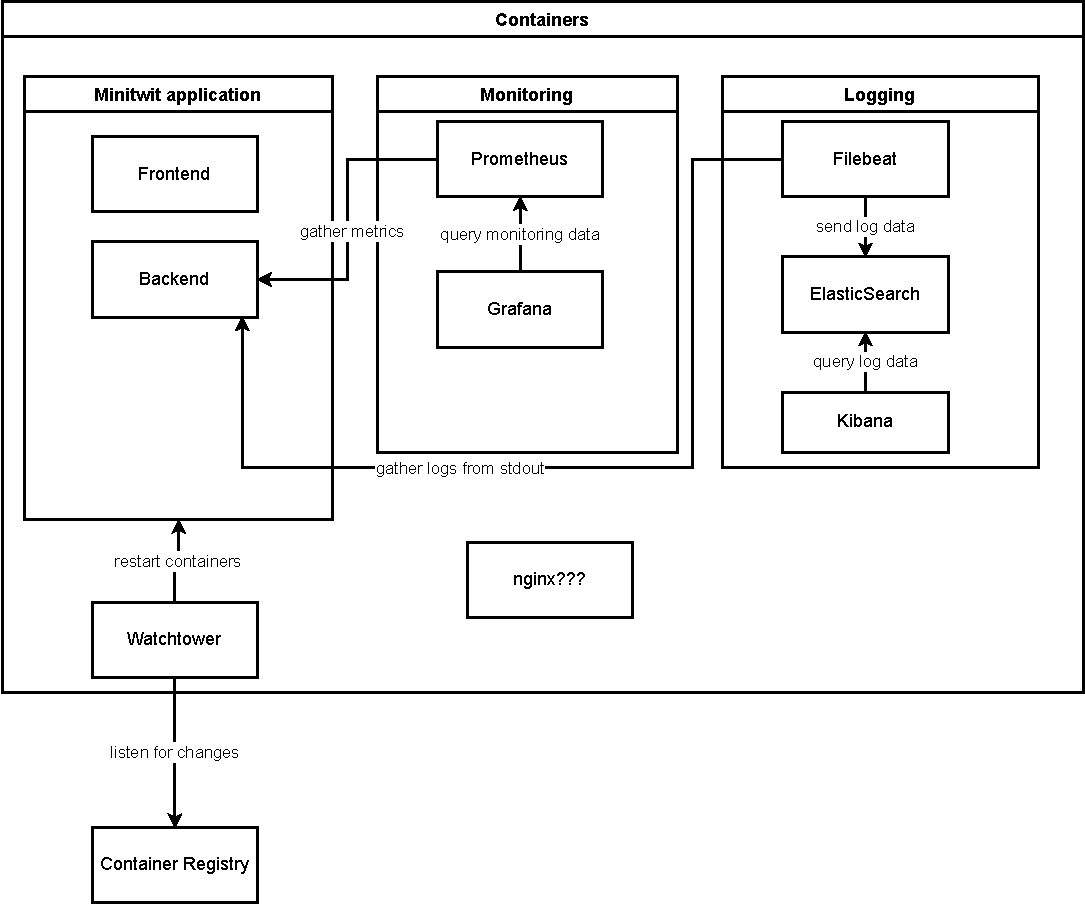
\includegraphics[scale=0.8]{report/diagrams/containers.pdf}
    \caption{Container overview}
    \label{fig:docker_containers}
\end{figure}

\subsection{Dependencies on all levels of abstraction}
\textbf{Hosting} depends on Virtual Machines (droplets) \& Database(postgres) managed by DigitalOcean. 
\\\\
\textbf{CI/CD chain} depends on Github Actions as a service Github runs. 
\\\\
\textbf{Remote code repository} is hosted on Github.
\\\\
\textbf{Docker installation} Our droplet installs docker through a script hosted at get.docker.com (Provided by docker themselves) if that script's contents were to change our behavior is undetermined.
\\\\
\textbf{Project dependencies:} Both the frontend and backend solutions rely on external dependencies and libraries in order to work. It is not feasible to construct every single package from the ground up, which is why we chose this approach. Since the frontend is build using Next.js we use npm as a package manager, which constructs a "package.json" that handles the dependencies. For the go backend, we also rely on external packages, that are all stored in a "go.mod" file. Both the "package.json" (\ref{subsec:package.json}) and "go.mod" (\ref{subsec:go.mod}) can be seen in the appendix.

\subsection{Current state of system}
% describe result of static analyis
To describe the state of the system, we have used SonarCloud's \cite{sonarcloud} service to review the code and quality of code. SonarCloud provides us with a series of reports, that indicate where possible security issues exists or where we have poorly written code. The results of the static code analysis is as follows\footnote{Full report can be found at \url{https://sonarcloud.io/project/overview?id=DevOps-CI-CDont_DevOps-CI-CDont2}}:
\begin{enumerate}
    \item 0 bugs
    \item 0 vulnerabilities
    \item 51 code smells (naming convention breaches, some things could be constants)
    \item 11 Security hotspots (eg. secrets in docker environment variables)
\end{enumerate}
A fix to the security hotspots would be to generate the environment secret for the docker-compose files through an external source, we have however not chosen to prioritize this task.

\subsection{License \& compatibility with direct dependencies}
The repository is provided with an MIT license \cite{mit_license}, which is an open-source license. This means that anybody that obtains a copy of our software is free to deal with the software without restrictions. This can impose problems on the direct dependencies that we use.
\\
Having an open-source MIT license can impose problems, as the package we are providing contains a bundle with direct dependencies. This issue can be mitigated, if all of our dependencies also have a MIT or similar open source license, which all of our dependencies have. The list of dependencies can be seen in \ref{subsec:package.json} and \ref{subsec:go.mod}
% not sure how to check this



\subsection{Choice of technologies}
\subsubsection{Frontend}
We chose Next.js as our frontend service, due to it's many build in features, such as:

\begin{enumerate}
    \item - Code splitting
    \item - Routing support
    \item- Server Side Rendering
    \item- Layouts and Components
    \item- API routes
    \item- Build in optimizations
    \item- Support for middleware
\end{enumerate}
Furthermore, we have added Tailwindcss as a CSS utility class for easy styling.
Having Server Side Rendering (SSR) isn't necessary for the Minitwit application, but it allows us to fetch data and build a page on the server, which gives a much better score on Google Lighthouse. Next.js also provides support for SEO optimizations, which is an important metric to be indexed and shown in Google searches. This is however, not important for this project.
\\
Having code splitting, divides the javascript build files into smaller files, making the size smaller and therefore 'lighter' to fetch, making the application faster.
\\
Next.js handles routing and API routes in the pages directory (Next.js 13 = app directory). This removes the overhead of having to create a React router that points to the different page components. Having a dedicated API routes folder, allows us to create API routes, that can fetch our backend data. The API routes folder removes many issues and privacy-related data, such as exposing environment variables.
\\
The Minitwit application has a user authentication system. With Next.js we can create a middleware that removes unauthenticated users from accessing pages, they're not allowed to view.
\subsubsection{API technology choice}
We chose to use Go with Gin to make a REST-ful API because:
It is a new language for all group members, so we can learn it together. We thought it would be an interesting language to build an API in. It is a pretty modern language, that is said to be built for concurrency, it's fast.  
*"The story goes that Google engineers designed Go while waiting for other programs to compile. Their frustration at their tool-set forced them to rethink system programming from the ground up, creating a lean, mean, and compiled solution that allows for massive multi-threading, concurrency, and performance under pressure\cite{stackoverflow2020golang}.
We first expected to use Go with Gorilla Mux, but we found out that that library has been archived - and so decided not to use Mux, and just decided to use Gin as it seemed popular, and provides the API tooling we thought was needed.
\subsubsection{Database}
At first we "inherited a local" database setup (a db file inside backend/tmp), and we didn't change that when we started containerizing the application. This was a very bad setup for real production data, as the database would be lost when the container was restarted. \\
We have since changed the database to a hosted PostgreSQL database via DigitalOcean. We chose to have the database maintained by a provider because the time we felt the time we would have to spend managing a database ourselves could be spent on more important parts of the project instead.
\subsubsection{Domain}
We used Name.com to purchase \url{cicdont.live} because they have a discount for a free year through github student pack. They point to nameservers on DigitalOcean, who then redirects to our droplet's specific IP. 

\subsubsection{DigitalOcean}
We chose DigitalOcean as our cloud provider simply because they provide \$200 worth of credit for students, and it was suggested in the course.

\subsubsection{Github Actions}
GitHub was already used as a remote git repository and as an issue-tracking platform. As it was also suggested by the course, we found it to be an easy choice to also use their platform for Continuous Integration and Continuous deployment. 

\subsection{Virtualization choices}
All the architecture that is needed to deploy the system, can be started from a single script in our repository.
The script requires a secret environment variable(API keys from digital ocean) that will allow the creation of droplets on our Digital Ocean account. From there we use Digital Ocean's CLI tool "Doctl" to create a ubuntu22-10x64 with 4 GB of RAM Virtual Machine hosted in France. The script then installs docker on the droplet before accessing our repository for configuration files through curl. Once all the necessary configuration files exist, we use docker-compose to run our service. Finally, we set up "iptables" that redirects http traffic (port 80) to the frontend (port 3000). 